% !TEX encoding = UTF-8 Unicode
%Encoding: UTF-8
\documentclass[toc=listofnumbered]{doku-tpl}

\usepackage{layout}
\usepackage{color}          			% Farben
\usepackage{colortbl}       			% Tabellen einfärben
\usepackage[utf8]{inputenc} 			% Encoding
\usepackage[binary-units=true]{siunitx}	% Einheiten
\usepackage{steinmetz}					% benötigt für Winkelzeichen \angle{}
\usepackage{amsmath, amssymb}			% Math
\usepackage{enumitem}
\usepackage{pdflscape} %\usepackage{lscape}
\usepackage{lmodern}
\usepackage{subcaption}
\usepackage{listings}
\usepackage{pdfpages}
\usepackage{titletoc}
\usepackage{pdflscape}
\usepackage{siunitx}
\usepackage[justification=centering]{caption}
\usepackage{bookmark}
\usepackage{booktabs}
\usepackage{threeparttable}

% Long/Short Version of documentation
\newif\iflong
\longtrue  % Confidential
%\longfalse  % Public
%  usage:
%  \iflong long version \else short version \fi 

% Row/Colspan Table
\usepackage{multirow,tabularx}
\newcolumntype{Y}{>{\centering\arraybackslash}X}
\renewcommand{\arraystretch}{2}

% Table Justification
\newcolumntype{L}[1]{>{\raggedright\let\newline\\\arraybackslash\hspace{0pt}}m{#1}}
\newcolumntype{C}[1]{>{\centering\let\newline\\\arraybackslash\hspace{0pt}}m{#1}}
\newcolumntype{R}[1]{>{\raggedleft\let\newline\\\arraybackslash\hspace{0pt}}m{#1}}

% Landscape
\def\insertpage{\mbox{}\vfil\hfil\thepage}

% Column sep in List of Abbreviations
\setlength\columnsep{30pt} % This is the default columnsep for all pages

% Big Frac
\newcommand\ddfrac[2]{\frac{\displaystyle #1}{\displaystyle #2}}

% Paragraph
\usepackage{amsthm}% for \@addpunct
\makeatletter
\def\els@aparagraph[#1]#2{\elsparagraph[#1]{#2\@addpunct{.}}}
\def\els@bparagraph#1{\elsparagraph*{#1\@addpunct{.}}}

% Footnote Einstellungen
\usepackage{footnote}
\makesavenoteenv{tabular}
\makesavenoteenv{table}
\usepackage[perpage, symbol, bottom]{footmisc}
\renewcommand{\thefootnote}{\fnsymbol{footnote}}

% Repeat figure caption
\usepackage{caption}
\newcommand{\repeatcaption}[2]{%
  \renewcommand{\thefigure}{\ref{#1}}%
  \captionsetup{list=no}%
  \caption{#2 (repeated from page \pageref{#1})}%
}

% "Evaluate at" math (vertical line) Example: |_{a}
\usepackage{amsmath,mleftright}
\usepackage{xparse}
\NewDocumentCommand{\evalat}{sO{\big}mm}{%
  \IfBooleanTF{#1}
   {\mleft. #3 \mright|_{#4}}
   {#3#2|_{#4}}%
}

% Math alphabet
\DeclareMathAlphabet{\mathpzc}{OT1}{pzc}{m}{it}

% Listings
\lstset{
    numbers=left,
    breaklines=true,
    tabsize=2,
    %basicstyle=\ttfamily,
    basicstyle=\footnotesize\ttfamily,
    literate={\ \ }{{\ }}1,
}
\lstloadlanguages{[Visual]Basic}

% Yaml Listings
\newcommand\YAMLcolonstyle{\color{red}\mdseries}
\newcommand\YAMLkeystyle{\color{black}\bfseries}
\newcommand\YAMLvaluestyle{\color{blue}\mdseries}
\newcommand\language@yaml{yaml}
\expandafter\expandafter\expandafter\lstdefinelanguage
\expandafter{\language@yaml}
{
  keywords={true,false,null,y,n},
  keywordstyle=\color{darkgray}\bfseries,
  basicstyle=\YAMLkeystyle,                                 % assuming a key comes first
  sensitive=false,
  comment=[l]{\#},
  morecomment=[s]{/*}{*/},
  commentstyle=\color{purple}\ttfamily,
  stringstyle=\YAMLvaluestyle\ttfamily,
  moredelim=[l][\color{orange}]{\&},
  moredelim=[l][\color{magenta}]{*},
  moredelim=**[il][\YAMLcolonstyle{:}\YAMLvaluestyle]{:},   % switch to value style at :
  morestring=[b]',
  morestring=[b]",
  literate =    {---}{{\ProcessThreeDashes}}3
                {>}{{\textcolor{red}\textgreater}}1     
                {|}{{\textcolor{red}\textbar}}1 
                {\ -\ }{{\mdseries\ -\ }}3,
}
\lst@AddToHook{EveryLine}{\ifx\lst@language\language@yaml\YAMLkeystyle\fi}
\newcommand\ProcessThreeDashes{\llap{\color{cyan}\mdseries-{-}-}}

% Capitalize TOC
%\usepackage{tocbibind}
%\let\oldaddcontentsline\addcontentsline
%\newcommand{\ADDCONTENTSLINE}[3]{%
%  \oldaddcontentsline{#1}{#2}{\MakeUppercase{#3}}%
%}
%\newcommand{\CAPinToC}{\let\addcontentsline\ADDCONTENTSLINE}
%\newcommand{\noCAPinToC}{\let\addcontentsline\oldaddcontentsline}


% Abbreviations with lowercase letters in text
\usepackage{acronym}
\usepackage{etoolbox}
\makeatletter
\newif\if@in@acrolist
\AtBeginEnvironment{acronym}{\@in@acrolisttrue}
\newrobustcmd{\LU}[2]{\if@in@acrolist#1\else#2\fi}
\newcommand{\ACF}[1]{{\@in@acrolisttrue\acf{#1}}}
\makeatother

% Json Listing
\usepackage{xcolor}
\definecolor{eclipseStrings}{RGB}{42,0.0,255}
\definecolor{eclipseKeywords}{RGB}{127,0,85}
\colorlet{numb}{magenta!60!black}
\lstdefinelanguage{json}{
    basicstyle=\normalfont\ttfamily,
    commentstyle=\color{eclipseStrings}, % style of comment
    stringstyle=\color{eclipseKeywords}, % style of strings
    numbers=left,
    numberstyle=\scriptsize,
    stepnumber=1,
    numbersep=8pt,
    showstringspaces=false,
    breaklines=true,
    frame=lines,
    backgroundcolor=\color{gray}, %only if you like
    string=[s]{"}{"},
    comment=[l]{:\ "},
    morecomment=[l]{:"},
    literate=
        *{0}{{{\color{numb}0}}}{1}
         {1}{{{\color{numb}1}}}{1}
         {2}{{{\color{numb}2}}}{1}
         {3}{{{\color{numb}3}}}{1}
         {4}{{{\color{numb}4}}}{1}
         {5}{{{\color{numb}5}}}{1}
         {6}{{{\color{numb}6}}}{1}
         {7}{{{\color{numb}7}}}{1}
         {8}{{{\color{numb}8}}}{1}
         {9}{{{\color{numb}9}}}{1}
}

% Listen-Item-Abstände global festlegen
\usepackage{enumitem}
\setlist[1]{itemsep=-4pt}

    % Eigene Tabellen
    % Hellgrau und weiss abwechselnd
\newenvironment{zebratabular}{\rule{0pt}{11pt}\rowcolors{2}{lgray}{white}\tabular}{\endtabular}
\newenvironment{zebralongtable}{\rule{0pt}{11pt}\rowcolors{2}{lgray}{white}\longtable}{\endlongtable}
\renewcommand{\arraystretch}{1.2}
\usepackage[babel,german=quotes]{csquotes}  % Deutsche Gänsefüsschen
\usepackage{acronym} 					% Abkürzungsverzeichnis
\usepackage{array,multirow,graphicx}		% Tabelle Multirow
%\usepackage[square, numbers]{natbib}
%\usepackage{makeidx}
%\bibliographystyle{abbrvnat}

\bibliographystyle{unsrtnat} 
\usepackage[sort&compress,numbers]{natbib}

\makeatletter

% Use stars in minipage footnotes
\renewcommand{\thefootnote}{\fnsymbol{footnote}}

\begin{document}

\newcommand\cntr{\centering\arraybackslash}
\renewcommand\STtextcell{@}
        
% no indent on newline
\setlength{\parindent}{0pt}
        
% display paragraph more like section
%\renewcommand\paragraph{%
% \@startsection{paragraph}{4}{0mm}%
%	{-\baselineskip}%
%	{.5\baselineskip}%
%	{\normalfont\normalsize\bfseries}}
%\makeatother
 
\subject{Master Thesis, FS20}
\title{Acoustic Scene and Room Classification for Real-Time Applications}
\subtitle{{\normalsize{Creation of Binaural Multi-Label Audio Dataset including Scenes and Soundscapes\\ \vspace{0.1cm} 
Training of Multi-Output Deep CNN in Python/Tensorflow with Keras\\ \vspace{0.1cm} 
Implementation Concept of Optimized CNN on Dedicated Hardware}}}
        \author{Silvio Emmenegger}
        \adviser{Prof. Dr. Jürgen Wassner}
        \data{Document classification: 
			\iflong Confidential \else Public \fi         
        \\ 
        \vspace{0.2cm} Horw, July 10, 2020}
        \frontpage{}
        
        \setcounter{page}{1}
        \pagenumbering{Roman}
 		\pagestyle{fancy}
 	 	
		\graphicspath{{img/}, {img/export/}} 
 		
 		% force fancyhdr on toc
 		\let\LaTeXStandardTOC\tableofcontents%
		\renewcommand{\tableofcontents}{%
		\begingroup
		\renewcommand{\thispagestyle}[1]{%
		\relax% Do nothing at all
		}%
		\LaTeXStandardTOC%
		\endgroup
		}%

        \renewcommand{\footrulewidth}{0.4pt}
        \pagebreak
		\fancyhead{}
	   	\fancyfoot{}	 
	 	\fancyhead[R]{Master Thesis, FS20}
	        
		\fancyfoot[L]{Silvio Emmenegger}
	  	\fancyfoot[C]{\thepage}
		\fancyfoot[R]{Hochschule Luzern T\&A}
    
        \fancyfoot[C]{Page \thepage \ of \pageref{LastPage}}
        
        \setlength{\headheight}{15pt}
        \setlength{\headsep}{0.2in}
         
        \setcounter{page}{1}
        \pagenumbering{arabic}
        
		% !TEX encoding = UTF-8 Unicode
%Encoding: UTF-8
\section*{Probity Statement}

% german
%\textit{Hiermit erkläre ich, dass ich die vorliegende Arbeit selbstständig angefertigt und keine anderen als die angegebenen Hilfsmittel verwendet habe. Sämtliche verwendeten Textausschnitte, Zitate oder Inhalte anderer Verfasser wurden ausdrücklich als solche gekennzeichnet.}

% english
\textit{I hereby declare that I have prepared the present work independently and have used no other than the specified aids. All used text excerpts, citations or contents of other authors were expressly marked as such.}
\\
\\
Horw, July 10, 2020
\\[2cm]
\begin{flushright}
    
\includegraphics[width=0.25\textwidth]{00_Sign.pdf}
    \\
    \vspace{-3mm}
	\@author
\end{flushright}	
		\clearpage
		\section*{Abstract}
Abstract text
		%    \include{content/abstract_de}

    	\clearpage
    	\vspace*{-10mm}
    	\tableofcontents
    	
%			  	
        \clearpage
        \fancyhead[L]{\partname \ \thepart \ - \parttitle}	  
        
        
%-----------------------------------------------------------------        
  		% Include Files
%-----------------------------------------------------------------        
  				
        \part{Introduction}
        % !TEX encoding = UTF-8 Unicode
%Encoding: UTF-8

        
\section{Initial Situation}

\subsection{State of the Art} 
Abbreviations of \ac{ADAM} or \aclp{CNN} (\acsp{CNN}) are introduced here. Sections can be referenced by Sec. \ref{sec:appdix_main_script}, while tables and figures can be referenced the same way (see Tab. \ref{tab:table1} and Fig. \ref{fig:figure1} or Fig. \ref{fig:figure2}).

\begin{figure}[htb!]
 \centering
 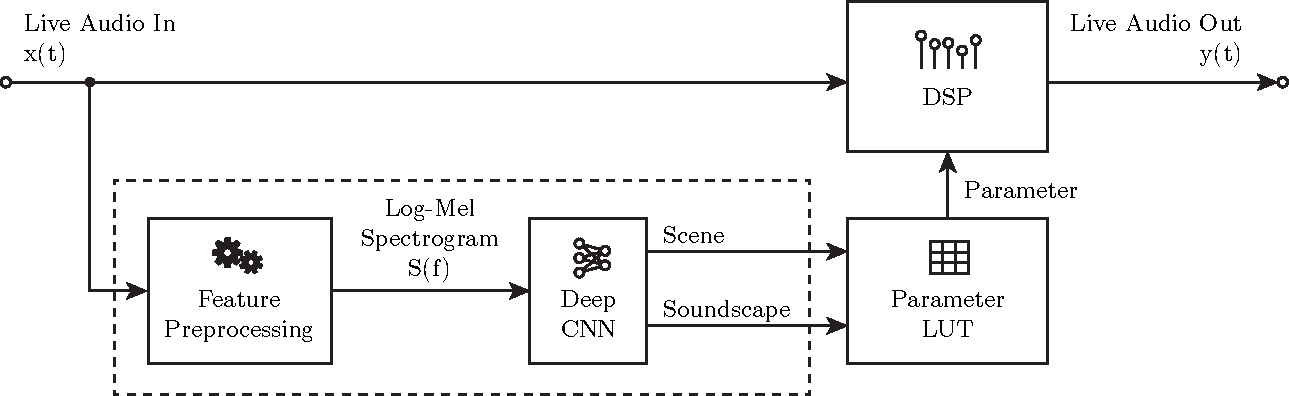
\includegraphics[width=0.85\textwidth]{01_Intended_System.pdf}
 \caption
 [Caption 1 in list of figures]
 {Caption 1 below figure \cite{axodraw}.}
 \label{fig:figure1}
\end{figure}

\begin{figure}[htb!]
 \centering
 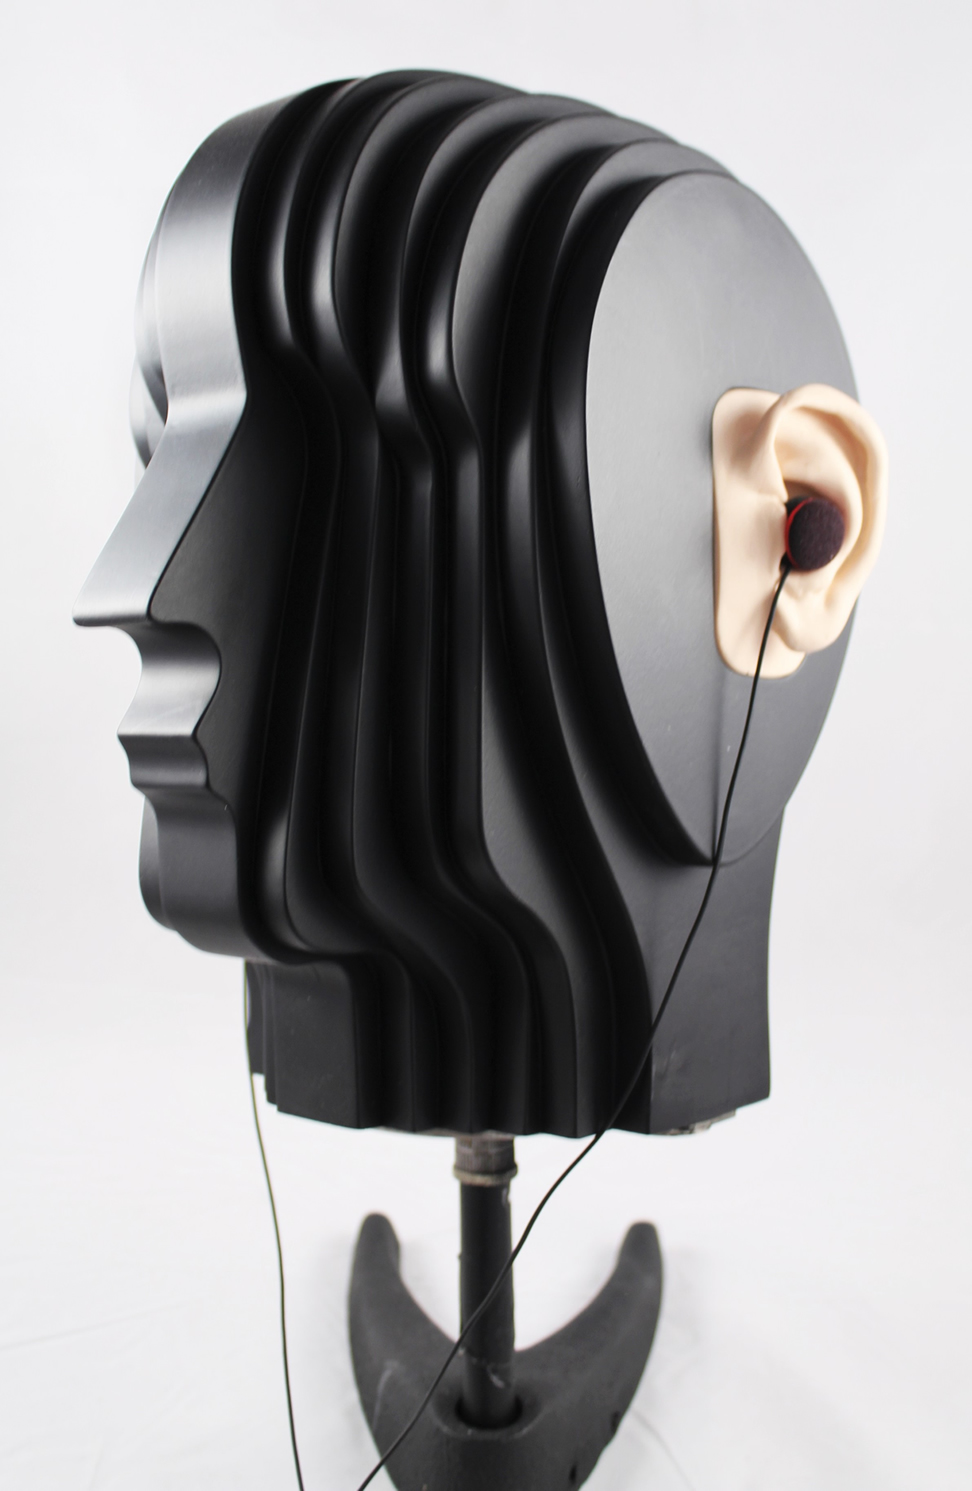
\includegraphics[width=0.15\textwidth]{02_DummyHead.jpg}
 \caption{Caption 2 below figure.}
 \label{fig:figure2}
\end{figure}

\subsection{Our Approach}


\newpage
\section{Project Scope}

\subsection{Time Horizon}

\subsection{Previous Work}

\subsection{Documentation Structure}

        \clearpage
        
        \part{Concept}
        % !TEX encoding = UTF-8 Unicode
%Encoding: UTF-8


\section{Problem Identification}
\label{sec:concept_problemident}

\begin{table}[h!]
 \centering
 \begin{tabular}{ L{3cm} C{4cm} R{3cm} } 
  \toprule
    \textbf{Col 1} & 
    \textbf{Col 2} & 
    \textbf{Col 3} \\
  \midrule
    left-aligned text & 
    centered text & 
    right-aligned text \\
  \bottomrule
 \end{tabular}
 \caption
 [Caption 1 in list of tables]
 {Caption 1 below table \cite{feynmf}.}
 \label{tab:table1}
\end{table}

As you can see, there are two captions. Maybe you want to add a reference in the caption below the table but not in the list of tables.

\subsection{Task Definition}
Information \footnote{Footnote text.}. \\
Text-variants:
\begin{itemize}
\item \textbf{bold font} 
\item \textit{italic font} 
\item \texttt{technical expressions} 
\item $\textsc{mathematical expressions such as} \hspace{3mm} T_{inf}$
\end{itemize}

\subsection{Real-Time Requirements}


\vspace{10mm}

\section{Existing Methods} 

\section{Chosen Approach}



        \clearpage
        
		\addtocontents{toc}{\protect\newpage}	% force newpage in toc
        \addtocontents{toc}{\protect\vspace*{2.5mm}}     % add vspace in toc
                
        \part{Realization}
        % !TEX encoding = UTF-8 Unicode
%Encoding: UTF-8

		
\section{Implementation}

\section{Evaluation}

\section{Demonstrator}



        \clearpage
        
        \part{Results}
        % !TEX encoding = UTF-8 Unicode
%Encoding: UTF-8

\addtocontents{toc}{\protect\newpage}			% force newpage in toc
        
\section{Results}

\section{Conclusion}

\subsection{Outlook}

        \clearpage
  
       
%-----------------------------------------------------------------        
  		% Verzeichnisse
%-----------------------------------------------------------------        
		
        \clearpage
		\fancyhead{}
	 	\fancyhead[R]{VM2, HS19}
	 	
	 	
		\bookmarksetup{startatroot} % next content out of last part in bookmarks
		
    	\clearpage
		\addcontentsline{toc}{section}{List of abbreviations}
    	% !TEX encoding = UTF-8 Unicode
%Encoding: UTF-8
\section*{List of Abbreviations}
\begin{multicols}{2}

    
\begin{acronym}[CC-IIMSN]

  	\setlength\itemsep{0.3em}  
  	
	% Singulars
	\acro{ADAM}{Adaptive Moment Estimation}
	\acro{CNN}{Convolutional Neural Network} 
	\acro{HSLU}{Hochschule Luzern} 
	
	% Plurals
	\acroplural{CNN}[CNNs]{Convolutional Neural Networks}

\end{acronym}
\end{multicols}	 	
    	
	 
        \addtocontents{toc}{\protect\vspace*{-2.5mm}}     % add vspace in toc
        
        
		%\section{Verzeichnisse}
		
		% Abbildungsverzeichnis
		
		%\addtocounter{subsection}{1}	
		%\addcontentsline{toc}{subsection}{\protect\numberline{\thesubsection}Abbildungsverzeichnis}
		\addcontentsline{toc}{section}{List of Figures}
		%\subsection{Abbildungsverzeichnis}
		
		\clearpage
%		\vspace*{-13mm}
		\vspace*{-21mm}
		\listoffigures
		
        \addtocontents{toc}{\protect\vspace*{-2.5mm}}     % add vspace in toc
        
        
		%\newpage
		
		% Tabellenverzeichnis    
		
		%\addtocounter{subsection}{1}	
		%\addcontentsline{toc}{subsection}{\protect\numberline{\thesubsection}Tabellenverzeichnis}
		\addcontentsline{toc}{section}{List of Tables}
		%\subsection{Tabellenverzeichnis}
		\listoftables
				
		
        \addtocontents{toc}{\protect\vspace*{-2.5mm}}     % add vspace in toc
        		
        
  		% Bibliografie
		\clearpage
		%\addtocounter{subsection}{1}	
		%\addcontentsline{toc}{subsection}{\protect\numberline{\thesubsection}Literaturverzeichnis}
 		%\addcontentsline{toc}{section}{\protect\numberline{Literaturverzeichnis}}
	   	\addcontentsline{toc}{section}{Bibliography}
	    %\lstlistoflistings
	    %\subsection{Literaturverzeichnis}
	    \renewcommand\refname{Bibliography}
	    \begin{flushleft}
	    	\bibliography{references}
	        \clearpage
	    \end{flushleft}
        \nocite{*} % alle quellen ausgeben


%-----------------------------------------------------------------        
  		% Appendix
%----------------------------------------------------------------- 
        
%	  	\fancyhead[L]{\partname \ \thepart \ - \parttitle}
	  	
	  	%\setcounter{figure}{0} \renewcommand{\thefigure}{A.\arabic{figure}}
	  	
%        \addtocontents{toc}{\protect\newpage}	% force newpage in toc
        \clearpage
%        \addtocontents{toc}{\protect\vspace*{-9mm}}     % add vspace in toc
        \part{Appendix}
		% !TEX encoding = UTF-8 Unicode
%Encoding: UTF-8

\appendix

%Der komplette Anhang befindet sich auf der beigelegten CD.
%\\

% OVERVIEW ABOUT APPENDIX ON CD
%\begin{multicols}{2}

\section{Attachments}
Following documents are attached at the end of this document:

\begin{itemize}
\setlength{\itemsep}{-2pt}
\item{000: Task Formulation}
\item{001: Research Plan}
\item{002: Project Plan}
\end{itemize}

For employees of \ac{HSLU}, all source code and calculation documents are available inside a GitLab repository on the Enterprise Lab servers:

\begin{itemize}
\item User access by request: \href{mailto:silvio.emmenegger@hslu.ch}{silvio.emmenegger@hslu.ch}
\item Current work: \href{https://gitlab.enterpriselab.ch/acoustics-ai/asrc-for-real-time-applications}{https://gitlab.enterpriselab.ch/acoustics-ai/asrc-for-real-time-applications}
\item Related work: \href{https://gitlab.enterpriselab.ch/acoustics-ai}{https://gitlab.enterpriselab.ch/acoustics-ai} 
\end{itemize}



\newpage
\section{Code snippets}

\subsubsection{Main script}
\label{sec:appdix_main_script}

\iflong {
\lstinputlisting[language=Python,
	caption={Python script.}, 
	captionpos=b, 
	label={lst:main}]{content/listings/main.py}

\newpage
}
\else
	(source code is confidential, only available to authorized persons)
\fi 

\subsubsection{Configuration Generator}
\label{sec:appdix_config_gen}
\iflong {
	
	\lstinputlisting[language={[Visual]Basic},
	caption={VBA script.}, 
	captionpos=b, 
	label={lst:config_gen}]{content/listings/main.vba}
	
}
\else
	(source code is confidential, only available to authorized persons)
\fi 




%% ###########################          ATTACHMENTS           ###########################


\includepdf[page={1,2,3}]{attachments/Aufgabenstellung_Masterthesis_SilvioEmmenegger.pdf}
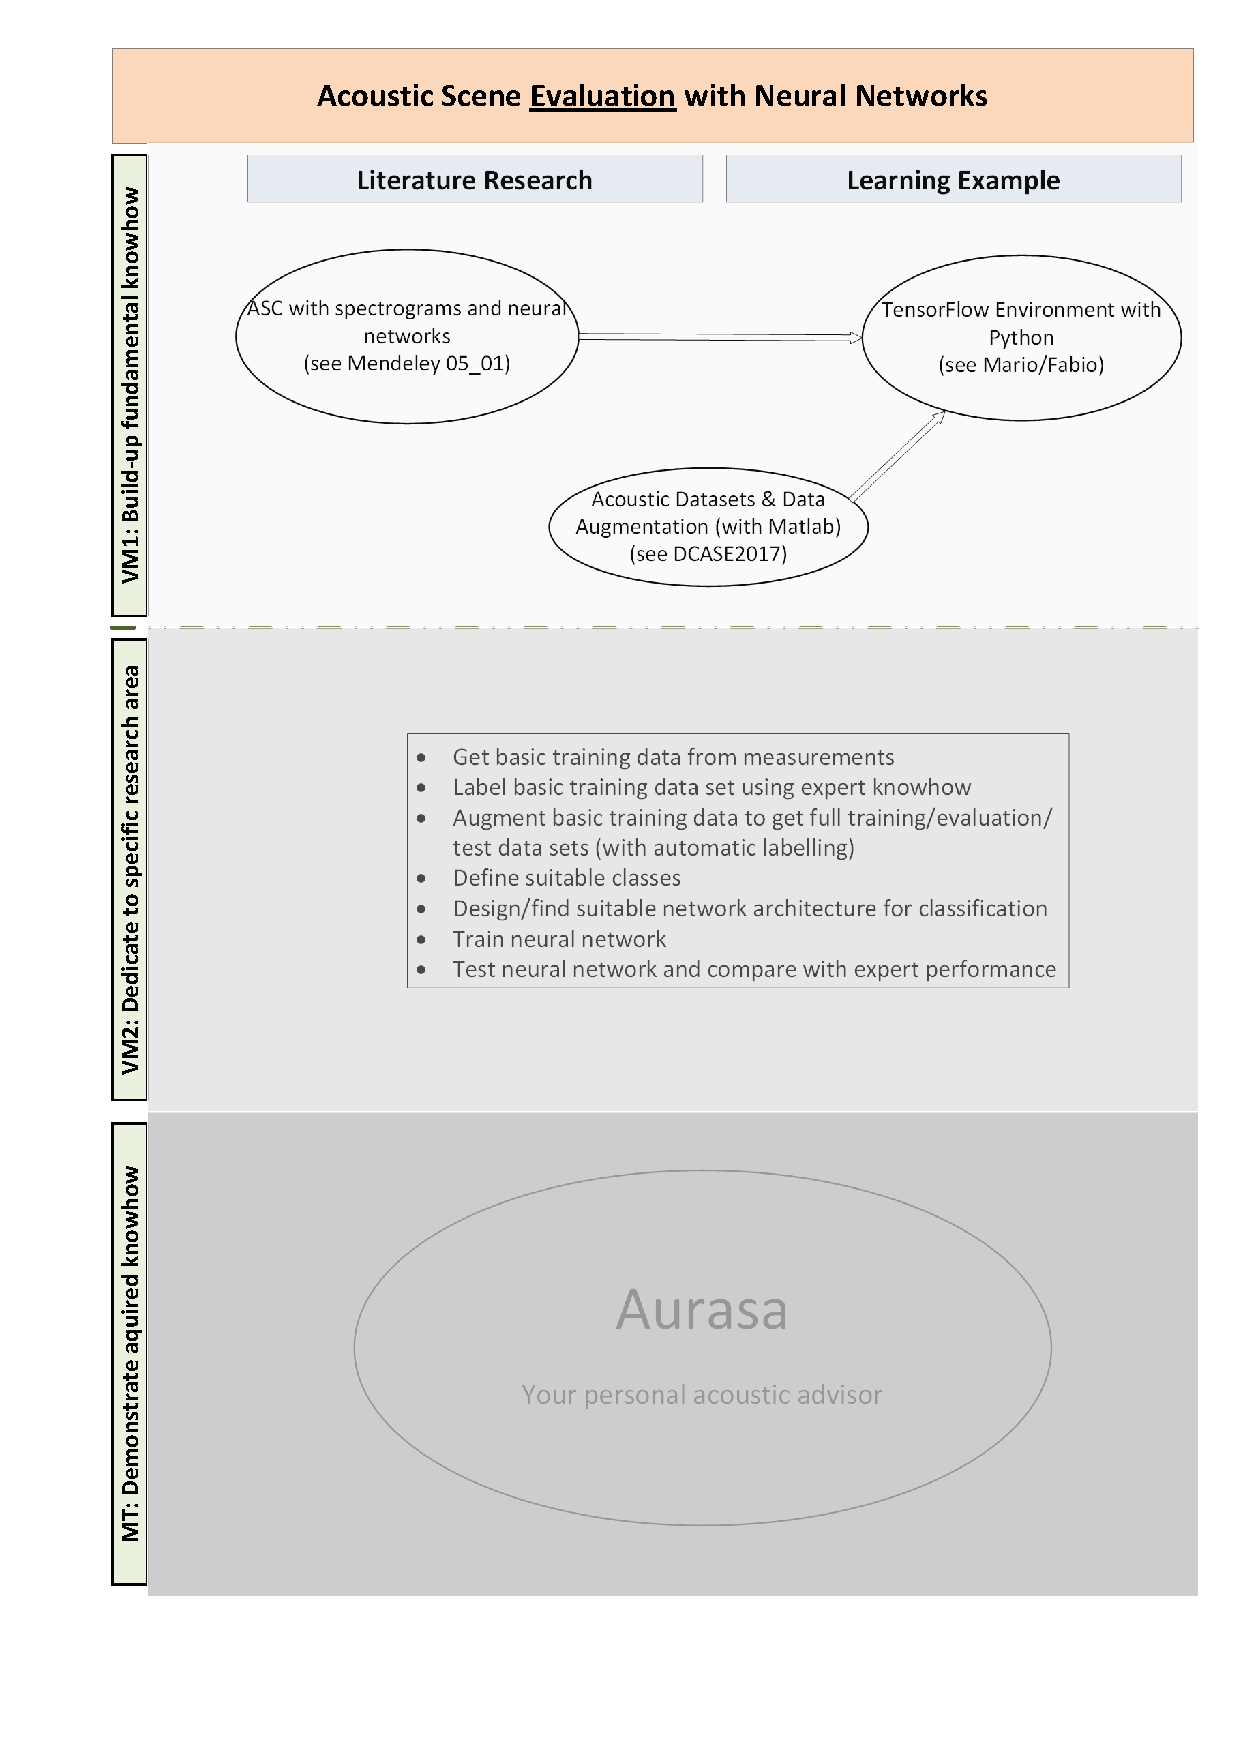
\includepdf[page={1,2}]{attachments/Research_Plan_Silvio_Emmenegger.pdf}
\begin{landscape}
	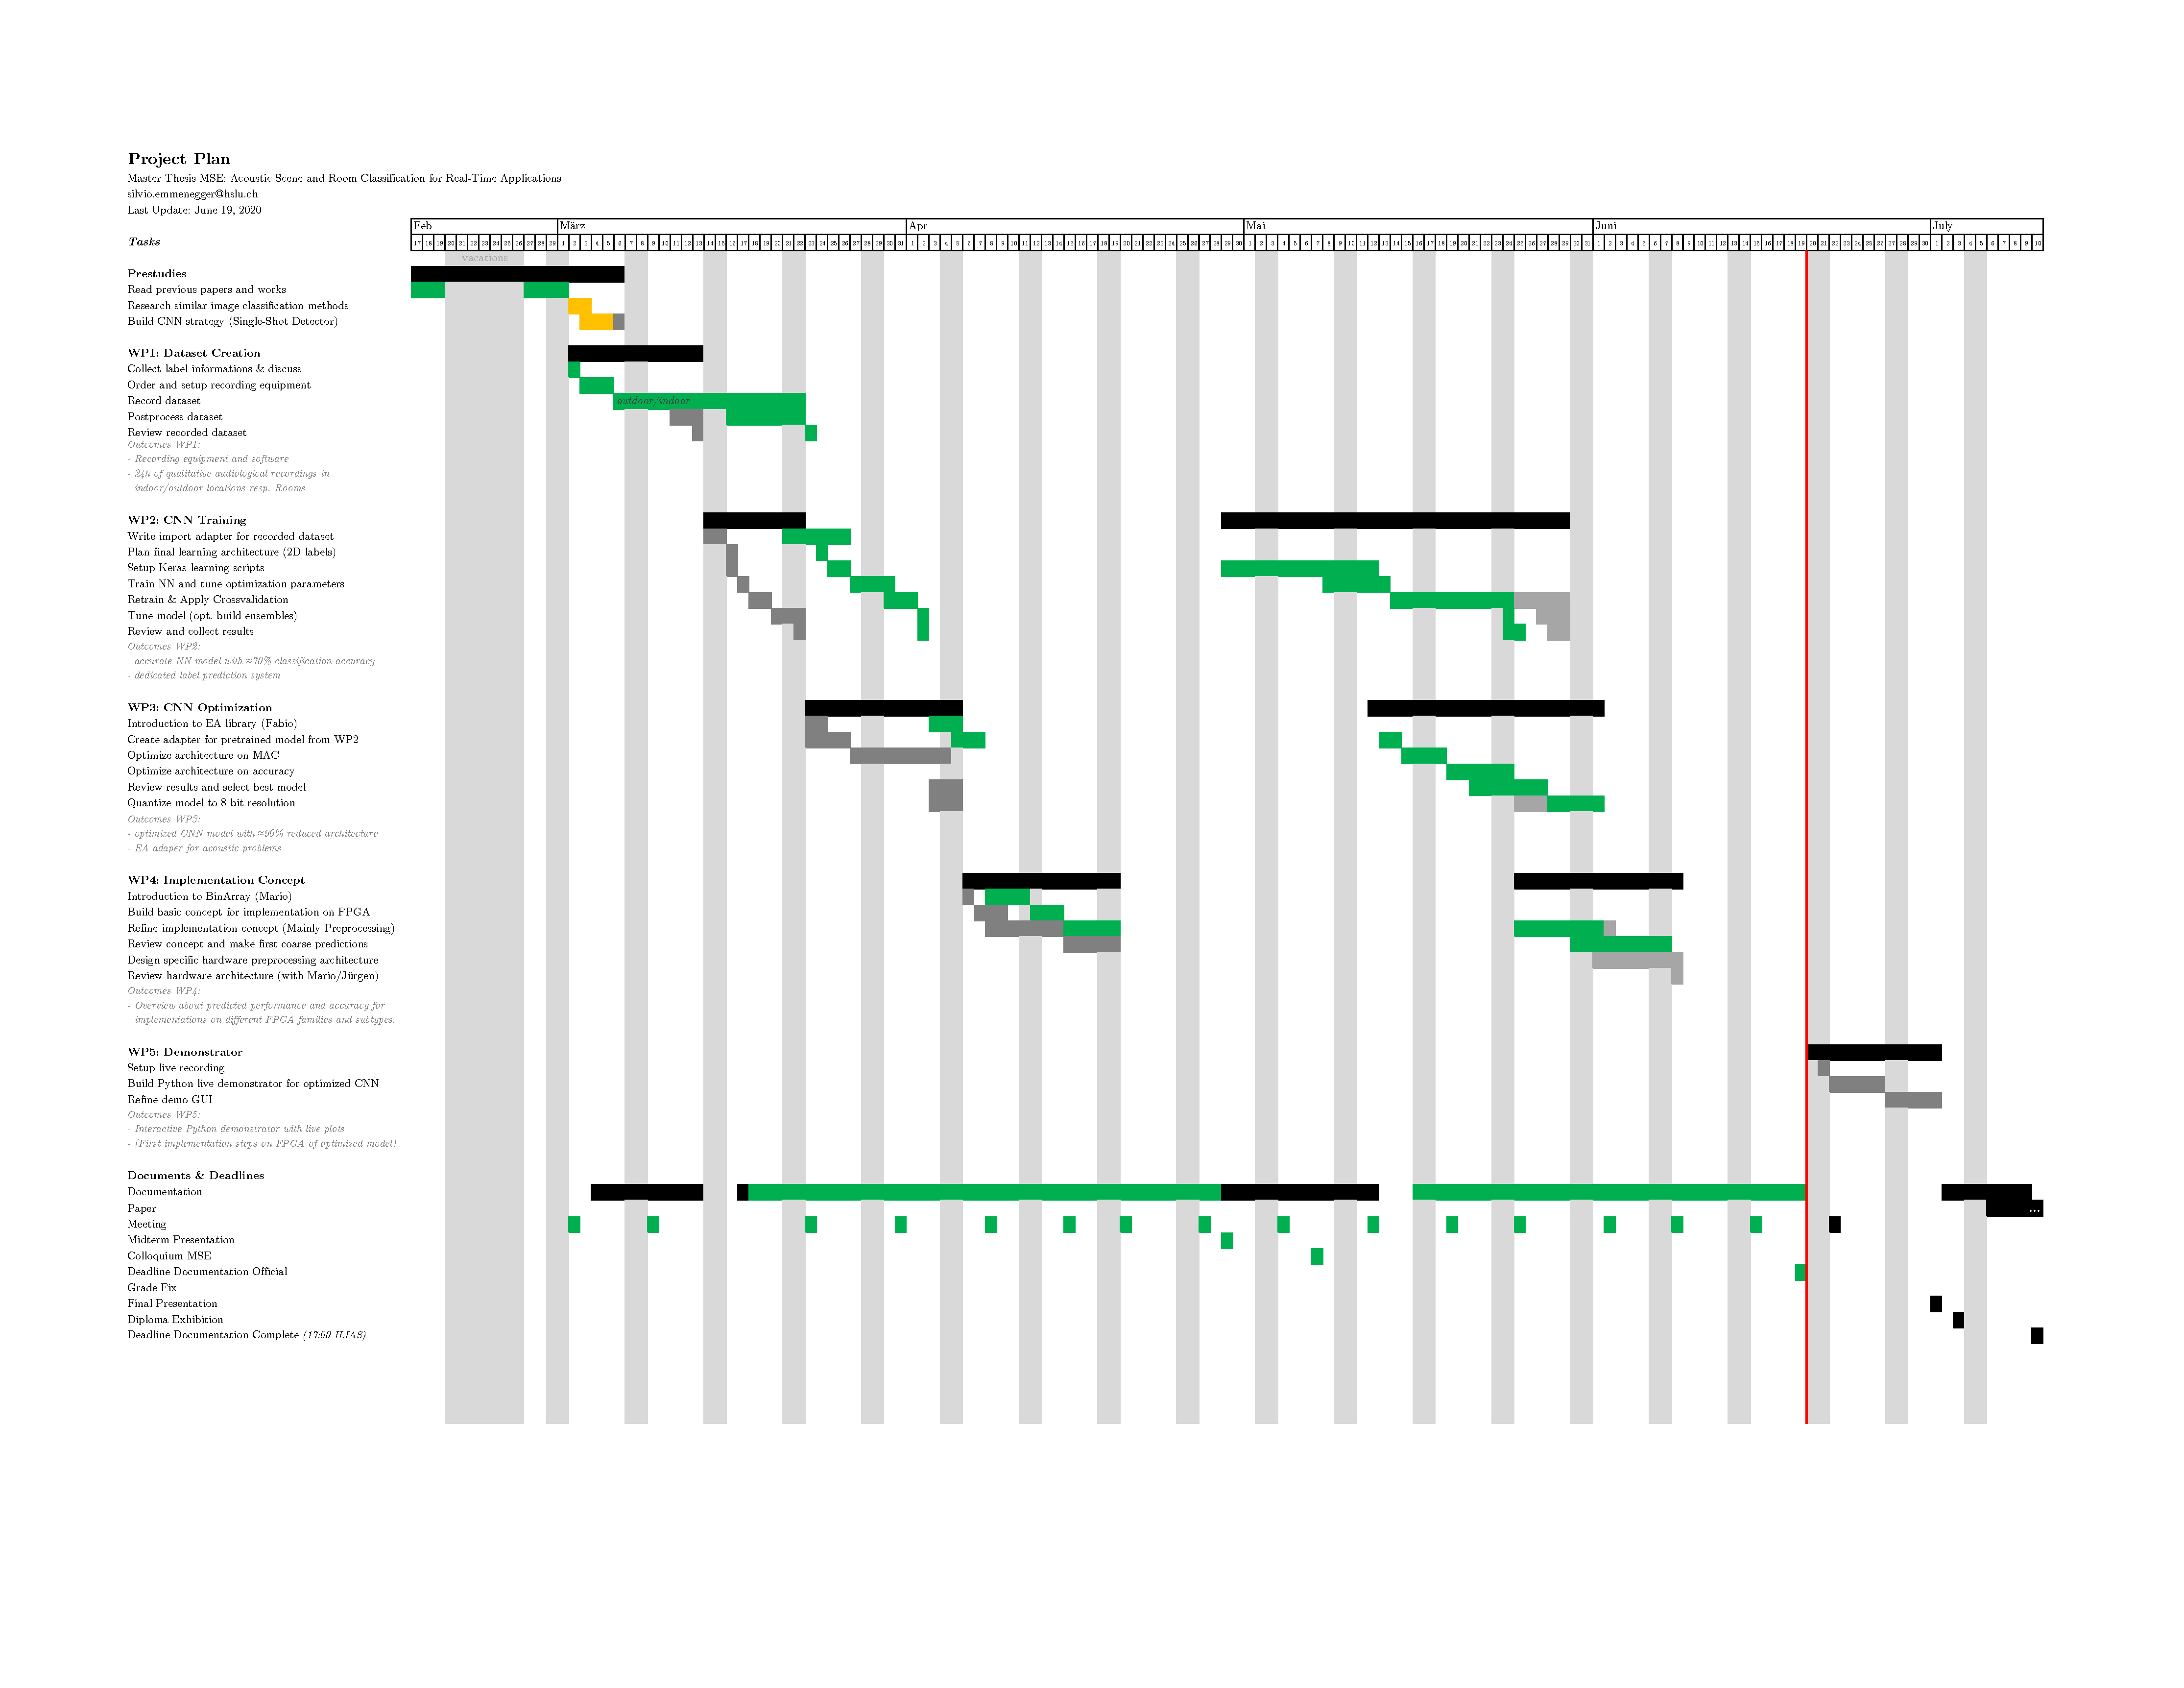
\includepdf[page={1}, landscape=true]{attachments/ProjectPlan_Detailed.pdf}
\end{landscape}
		
%		\addcontentsline{toc}{section}{List of listings}

%		\lstlistoflistings
        
       	% \pagenumbering{gobble}
        \fancyhead[L]{\nouppercase\rightmark}
        	\fancyfoot[C]{}
        	\fancyfoot[L]{Silvio Emmenegger}
        \fancyfoot[C]{Seite \thepage \ von \pageref{LastPage}}
        	\fancyfoot[R]{Hochschule Luzern T\&A}
        
        \titleformat{\section}
        [display]
        {\normalfont\Huge\bfseries\centering\vspace*{7cm}}
        {\titlerule[2px] \vspace{20px}\appendixname \ \thesection}
        {0pt}
        {\huge}[\rule{\textwidth}{2px}]
	
        
        \include{content/appendix}  
    
\end{document}